\section{Task Planning (Jim)}

The high-level planner in this work serves as the ``brain'' of the whole framework.
It takes an input of the {\it configuration file} and automatically generate and execute an assembly plan to place given modules as specified in the {\it configuration file}.
Fig.~\ref{fig:taskplan} shows the overview structure of the high-level task planner.

\begin{figure}[ht!]%[H]
\centering
{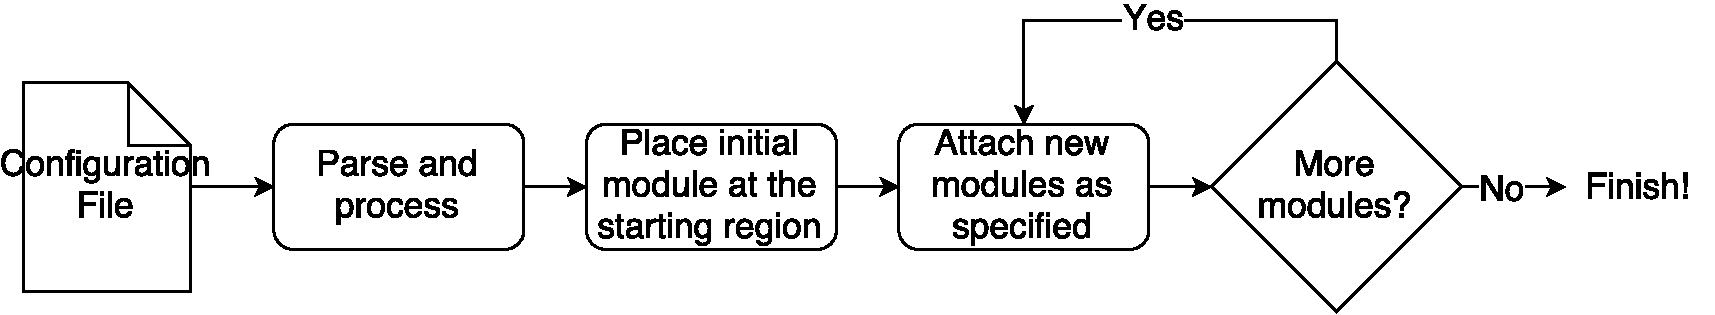
\includegraphics[width=0.95\columnwidth]{pics/highlevelflow.pdf}}
\caption{High-level Task Planning Module}
\label{fig:taskplan}
\end{figure}

\subsection{Parse and process the configuration file}
To specify the desired configuration of the modular robots, a user can use an existing designer VSPARC ({\color{red}cite}) to design the configuration and generate a {\it configuration file} that encodes information of the connectivity among all modules.
Fig.~\ref{fig:configfile} shows an sample {\it configuration file}.

\begin{figure}[ht!]%[H]
\centering
{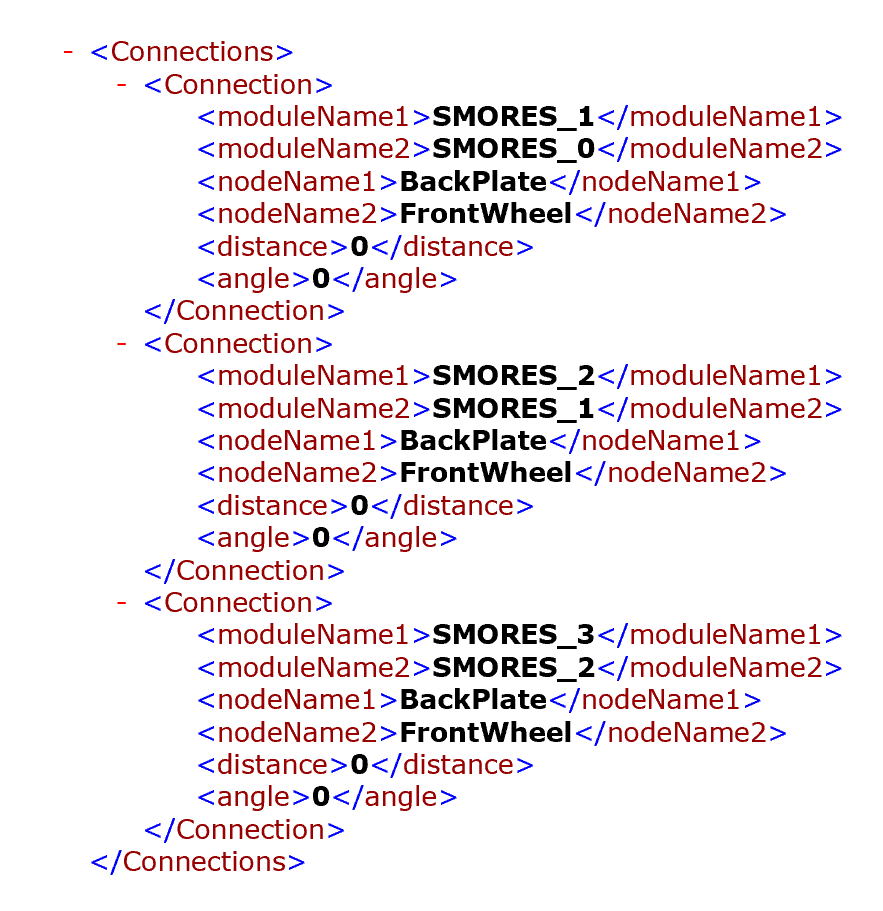
\includegraphics[width=0.95\columnwidth]{pics/configfile.png}}
\caption{A sample configuration file}
\label{fig:configfile}
\end{figure}

The high-level planner can parse the {\it configuration file} and build a graph encodes all connections.

\subsection{Place initial module at the starting region}
To start the assembly, an initial module needs to be selected and placed at the starting region.
\subsubsection{Select initial module}
Consider the scenario shown in Fig.~\ref{fig:loop}. Eight modules are placed at locations in blue.
It is hard to place a new module at the center location in red, as it is  fully surrounded by eight modules. Therefore, we decide to assemble modules in the order such that modules located in the center of the configuration are placed before modules located at edges of the configuration.
To achieve this guarantees, we rank all modules based on the number of connections each module has. The maximum connection a module can has is four.
Therefore, all modules are separated into four ranks. The higher the rank, the more connections a module has. 
When choosing the initial module, we will prefer the module in a higher rank. 
If there are more than one module in a rank, we will prioritize the module with more high rank neighbors.
This selection method is also utilized when choosing the next module to be placed as describe in Section~\ref{sec:nextmodule}.
With this ranking method, we might still encounter difficulty when solving the scenario in Fig.~\ref{fig:loop2}.
For example when the configuration is a 7-by-7 square made of 49 modules, we do not have difference in preference among modules in red.
In this work we only consider small size configurations (under 10 modules). Therefore the situation in Fig.~\ref{fig:loop2} will not happen.

\begin{figure}[ht!]%[H]
\centering
{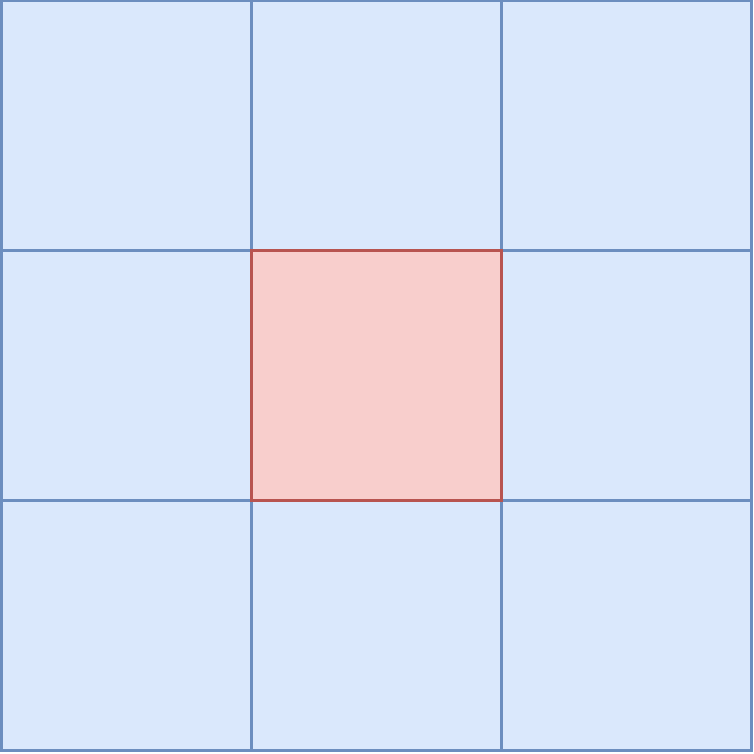
\includegraphics[width=0.3\columnwidth]{pics/moduleloop.pdf}}
\caption{A difficult scenario for adding a new module at red location}
\label{fig:loop}
\end{figure}

\begin{figure}[ht!]%[H]
\centering
{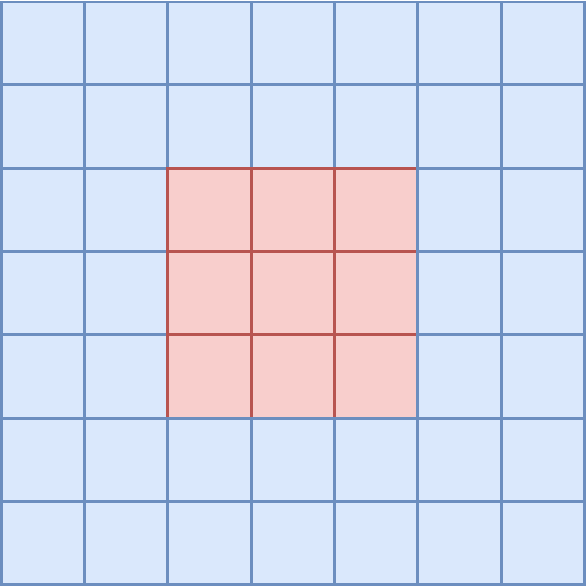
\includegraphics[width=0.3\columnwidth]{pics/moduleloop2.pdf}}
\caption{Modules in red cannot be distinguished}
\label{fig:loop2}
\end{figure}

\subsubsection{Search for starting region}
The starting region of the task is labeled with an AprilTag with an unique ID. Using the external camera, the task planner is able to find the positions and orientation of the starting point in the robot workspace. In this work, we choose the starting region to maximize the working area of the robot.

\subsubsection{Place the initial module to the starting region}
With the initial module and the starting region identified, the high-level planer then invoke the trajectory planner to control the robot to pick up the module and place it in the starting region.
When picking up a module, if the robot fails to grab the module, the task planner will receive the failure status from the trajectory planner and inform the user. The user can choose to retry or abort the task.

\subsection{Attach new modules}
Once the initial module in place, the task planner will continues to attach more modules as specified in the {\it configuration file} until the configuration is completed. To attach each module, the high-level planner will go through a sequence of actions as illustrated in Fig.~\ref{fig:attach}.

\begin{figure}[ht!]%[H]
\centering
{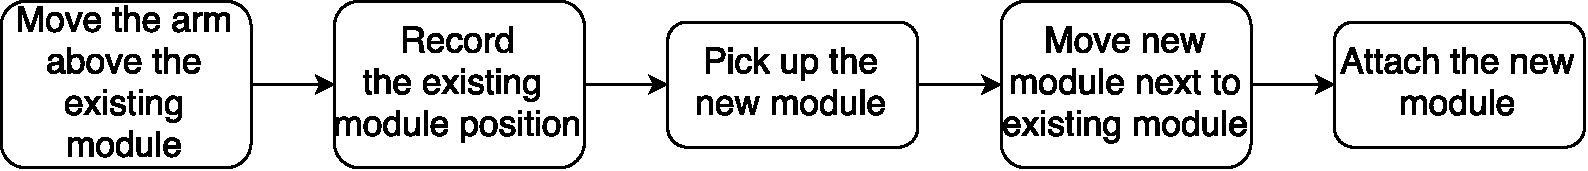
\includegraphics[width=0.95\columnwidth]{pics/attach.pdf}}
\caption{Sequence of actions when attaching a new module to existing modules}
\label{fig:attach}
\end{figure}

\subsubsection{Select the existing and new module}\label{sec:nextmodule}
As described in the previous section, we apply special preference when planning the assembly sequence, in order to avoid difficult manipulation scenario.
Different from choosing the initial module, when choosing an existing module, we only consider those that are already connected to the initial module.
With an existing module, the task planner chooses a new module that needs to be connected to the existing module based on the {\it configuration file}.

\subsubsection{Move the arm above the existing module and record its position}
When the robot arm successfully picked up a module, the module will block the view of the camera on the arm.
Since the trajectory planner needs to use the camera for localizing the position of the module, that task planner will first localize the existing module before picking up the new module.
In order to localize the existing module, the high-level planner will invoke the trajectory planner to move the arm roughly above the existing module, where the camera on the robot arm can get a updated and more precious position of the existing module.
This position is then recorded for later reference.

\subsubsection{Pick up the new module and move it next to the existing module}
After locating the existing module, the high-level task planer then ask the trajectory planer to control the robot arm to pick up the new module.
To prepare for attaching the new module, the new module needs to be close to the existing module.
This is achieved by moving the arm to a position slightly shifted from the previously recorded existing module position.

\subsubsection{Attach the new module to the existing module}
With the new module being next to the existing module, the high-level planner then call the action planner to generate and perform a verified controller to slowly move and attach the new module to the existing module.

\subsection{Future work: Synthesize the sequence of actions with formal method}
Inspired by the framework introduced in \cite{HKG2009}, we would like to implement a controller synthesis algorithm in the high-level task planner to automatically generate the action sequence shown in Fig.~\ref{fig:attach} from reactive robot task specifications.
A reactive robot task specification is expressed in LTL formulas.
Then the specification is automatically transformed to a correct-by-construction discrete controller.
At last, the controller can be continuously implemented to generate desired robot behaviors.
Using formal method, the high-level task planner will be able to inform the user if there is potential failure in the specified tasks.



%Therefore, there are three main challenges in this work for task planning, as described in the following sections.
%
%\subsection{Specification Language for Multi-robot}
%In \cite{ChenDSB12,Diaz-MercadoJBE15}, the author introduces an approach for specifying robot tasks in formal language and generating controllers for a team of robots. 
%However, the type of robot tasks is limited to non-reactive, i.e. the environment is assume static and the robot behavior does not depend on the environment state.
%The framework in \cite{HKG2009} allows reactive robot task, such as "if the robot sense a soda can, bring the can to the kitchen".
%However, the task specification only issues commands for a single robot.
%In order to specify reactive tasks for a team of robots, we need to extend the specification language to able to express  multi-robot tasks.
%
%\subsection{Tasks Allocation}
%The framework employed in this work will generate a centralized controller for a team of robots.
%We will then distribute tasks to each robots in a synchronized process.
%One method is to handle task allocation in the high-level specification.
%Therefore, task distribution for each robot will be encoded in the synthesized controller.
%The drawback for this method is that, whenever a new task allocation is required,
%possibly due to failing to find a feasible trajectory, the entire discrete controller needs to be resynthesized.
%Another method for task allocation is to treat all robots as one virtual robot with multiple redundant action abilities.
%The specification will only describe tasks for this virtual robot,
%and the task allocation will be determined when executing the synthesized controller.
%The disadvantage of this method is that the algorithm will spend more time during execution for computing the task allocation plan.
%Both method will be implemented in this work.
%We will compare the performance of both methods and choose the better one.
%
%\subsection{Feedback from Trajectory Planner}
%Once task are allocated to each robot, the task planner will invoke the trajectory planner to move each robot arm to desired location without collision.
%In the situation where the trajectory planner fails to find a feasible path for an arm,
%it will provide feedback to the task planner about such failure.
%The task planner will then incorporate the information into the task specification and come up with a new discrete plan.
%If no plan can be created, the task planner will notify the user the possible cause of failure, e.g. the robot arm cannot reach the desire position. 